\documentclass[12pt]{article}

\usepackage{sbc-template}
\usepackage{graphicx,url}

%\usepackage[brazil]{babel}   
\usepackage[utf8]{inputenc}  
\usepackage{pgfgantt} % For Gantt charts
\usepackage{enumitem}

\sloppy

\title{Analysis of Communities formed on Youtube Comment Sections}

\author{Thiago Amado Costa\inst{1}, Humberto Torres Marques Neto\inst{1}}


\address{ICEI – Pontifícia Universidade Católica de Minas Gerais (PUC-MG)\\
    Belo Horizonte, Minas Gerais - Brasil \email{thiago.amado@sga.pucminas.br, humberto@sga.pucminas.br} }

\begin{document}

\maketitle

\begin{abstract}
    YouTube is the largest video streaming platform on the web, attracting billions of users 
    daily who watch and engage with content through comments. 
    A significant portion of these users consists of children and teenagers, who frequently interact 
    with one another in the comment sections, forming active communities. 
    However, these communities can also experience negative interactions between users, 
    including instances of online bullying and hate speech.
    To explore these communities, the YouTube Data API v3 was used to collect comments 
    from videos produced by creators targeting this demographic. 
    Topic modeling and sentiment analysis were then applied to further explore the 
    content and dynamics within these communities.
\end{abstract}

\section{Introduction}
% >> Descrição de motivações
% >> Problema escolhido e objetivos

% - youtube
% - kids, teenagers 
% - brasil 
% - bullying, 
% - comentarios, comunidades 

Youtube has grown exponentially since its launch in 2005. With billions of users, it is now the 
largest video streaming platform on the web, and and a major source of online entertainment content. 
As mentioned by \cite{app13064044}, many children and teenagers use the platform as an alternative to 
traditional entertainment sources, such as television, with the majority of their 
browsing time spent on YouTube.

One of the ways kids and teenagers interact on the platform is through the comment section. 
This feature allows users to share their thoughts on the video, the content creator, 
or even other commenters. Additionally, users can respond to existing comments, 
facilitating public conversations and discussions on a wide range of topics, forming community structures. 
Unfortunately, many users take advantage of this feature to spread negative comments, targeting 
either the content creator or other commenters. 
This can lead to a toxic enviroment which is particularly concerning given the platform's 
popularity among children and teenagers.

Therefore, this study aims to analyze the community structures that emerge within the comment 
sections of Brazilian YouTubers who create content aimed at children and teenagers, 
as well as the content of the comments themselves.

\section{Related Work}

Identifying and mitigating the spread of toxicity on online platforms has become a pressing concern 
in recent years, as the proliferation of social media platforms has enabled the rapid dissemination of
bullying, hate speech, and other forms ot toxic behaviour.
In this section, we review existing research that focuses on community detection on social media,
as well as textual content analysis.


\cite{shajari2023} explores the problematic behaviors of 
commenters on YouTube, specifically focusing on "commenter mobs" that manipulate engagement 
metrics to distort public perception, particularly around misleading narratives about the U.S. military. 
By analyzing 20 targeted channels through social network analysis, the research fills gaps in 
understanding how suspicious commenter activities boost engagement, which has been insufficiently 
addressed in prior literature. Employing a co-commenter network model and clustering techniques, 
the study identifies distinct groups with varying levels of suspiciousness and highlights collusion 
among commenters across channels. Key findings reveal central figures driving discussions and 
coordinated efforts to amplify specific narratives, suggesting these channels significantly contribute 
to the spread of misinformation. The study concludes with a call for further research into the 
motivations behind these behaviors and their implications for misinformation dissemination online.


\cite{hussain2018analyzing} examines how the proliferation of smart devices and social media, 
particularly YouTube, has facilitated social and political fragmentation through cyber propaganda,
especially targeting youth with conspiracy theories. 
It investigates disinformation tactics used on a specific conspiracy theory channel,
distinguishing its approach from previous studies by focusing on user engagement patterns rather 
than just spam detection. 
Data was collected using the YouTube Data API, monitoring metrics like views, likes, dislikes, 
and comments, revealing patterns indicative of potential manipulation. 
The analysis identified two commenter groups, peripheral and core, with the second group exhibiting higher 
instances of inorganic behaviors. A co-commenter network analysis revealed clusters around specific 
conspiracy topics and identified bot-like and spam actions. The study emphasizes the need for early 
detection of such behaviors to safeguard democratic processes and suggests future research on 
comment semantics and algorithmic biases in video recommendations.


\cite{ashraf2021abusive} addresses the growing issue of abusive language on social media, 
particularly YouTube, highlighting its mental health implications and the urgent need for 
effective detection models. It reviews various abusive language datasets, including the Smokey-Corpus 
and Twitter-WH-Corpus, and contrasts early detection methods with recent advances in machine 
learning and deep learning techniques that incorporate contextual information. The authors present 
a novel dataset of 18,794 YouTube comments and replies, emphasizing a context-aware approach 
to labeling abusive language, with a focus on political and religious topics. 
The study highlights the importance of context in accurately detecting abusive language 
and notes challenges related to non-standard language forms, suggesting directions for 
future research that includes expanding the dataset and employing advanced classifiers like BERT.


\cite{kirdemir2023} investigates coordinated inauthentic campaigns on YouTube, focusing on 
characterizing suspicious behaviors through a multi-step analysis of engagement trends and co-commenter 
networks.  
Data was collected from 39 channels over several years, with an emphasis on identifying anomalous 
behaviors through rolling window correlation analysis and a long short-term memory (LSTM) model to 
generate suspicion scores. The findings reveal patterns indicative of manipulation, such as increasing 
views paired with decreasing subscribers, and highlight channels exhibiting coordinated 
commenting behaviors. The study concludes with a call for enhanced detection methodologies that 
integrate these findings to effectively counteract harmful campaigns on the platform.


\cite{shekar2021} investigates the prevalence and nature of abusive comments on YouTube, 
particularly focusing on the impact of hate speech on users, especially teenagers. 
Utilizing exploratory data analysis and topic modeling, the research aims to identify patterns of 
abuse and the most affected content creators by manually labeling a custom dataset due to the lack 
of publicly available resources. Data was collected from selected YouTube celebrities using the 
YouTube Data API, and a thorough cleaning process resulted in a Document Term Matrix for analysis. 
The study employed Latent Dirichlet Allocation (LDA) for topic modeling and sentiment analysis using 
the TextBlob library to assess the emotional tone of comments. Findings revealed that certain 
YouTubers received significantly harsher comments, with varying sentiment levels indicating the 
need for interventions to protect young creators from severe online harassment. 
The study concludes by recommending measures such as disabling comments on particularly abused 
videos and emphasizes the importance of understanding the dynamics of cyberbullying.

\section{Methodology}

This study uses a similar methodology as previous works. It consists of a data collection phase, 
a community analysis phase, and a content analysis phase.

\subsection{Data Collection}

Initially, the YouTube Data API v3 was used to gather comprehensive channel metadata for each 
specific YouTuber. Subsequently, we retrieve the IDs and titles of 50 videos from each channel. 
Finally, we construct the YouTuber's comments dataset by aggregating all comments and replies 
associated with each video, as well as the author information and the number of likes of each comment. 

As a preliminary analysis, the study focused on two YouTubers: Felipe Neto, who has 46.6 million 
subscribers, and Enaldinho, with 38.7 million subscribers. A total of 43,232 comments were collected 
for Felipe Neto, while 26,702 comments were gathered for Enaldinho. From this point on, they will
be called Youtuber 1 and Youtuber 2.

\subsection{Community Analysis}

To analyze the communities that emerge within each YouTuber's comment section, the dataset constructed 
in the previous phase is used to develop two networks: the video-commenter network and 
the co-commenter network, as demonstrated by \cite{hussain2018analyzing}. The video-commenter network 
is established by linking each commenter to the respective video on which they commented. 
In contrast, the co-commenter network is formed by connecting two commenters who have engaged with 
the same video. These networks facilitate the identification and examination of highly engaged users, 
as well as users exhibiting suspicious behaviors.

\subsection{Content Analysis}

Following the construction of the Co-Commenter Network and the Video-Commenter Network, we implement
topic modeling and sentiment analysis. For the topic modeling phase, we employ the BERTopic model 
(\cite{bertopic2022}), while the sentiment analysis is conducted using the multilingual 
XLM-roBERTa-base model (\cite{barbieri-etal-2022-xlm}). 
Initially, the comments are processed and cleaned, masking user handles to preserve anonymity,
removing emojis, links and stopwords
Then, topic modeling is utilized to extract themes associated with the communities identified in the 
previous phase. Finally, the sentiment analysis model evaluates the polarity of the content, 
offering deeper insights into the emotional tone of the discussions and facilitating a more 
comprehensive analysis of the identified topics.


\section{Early Results}

In this section, the early results are shown and commented.

After building the commenter networks, visualization methods were used for analysis.
In Figure~\ref{fig:ytbr1_vc_net}, red nodes are commenters and green nodes are videos they commented on.
The visualization clearly distinguishes between more engaged users, 
located within the central cluster, and less engaged users, situated in the outer clusters.

\begin{figure*}[t!]
    \centering
    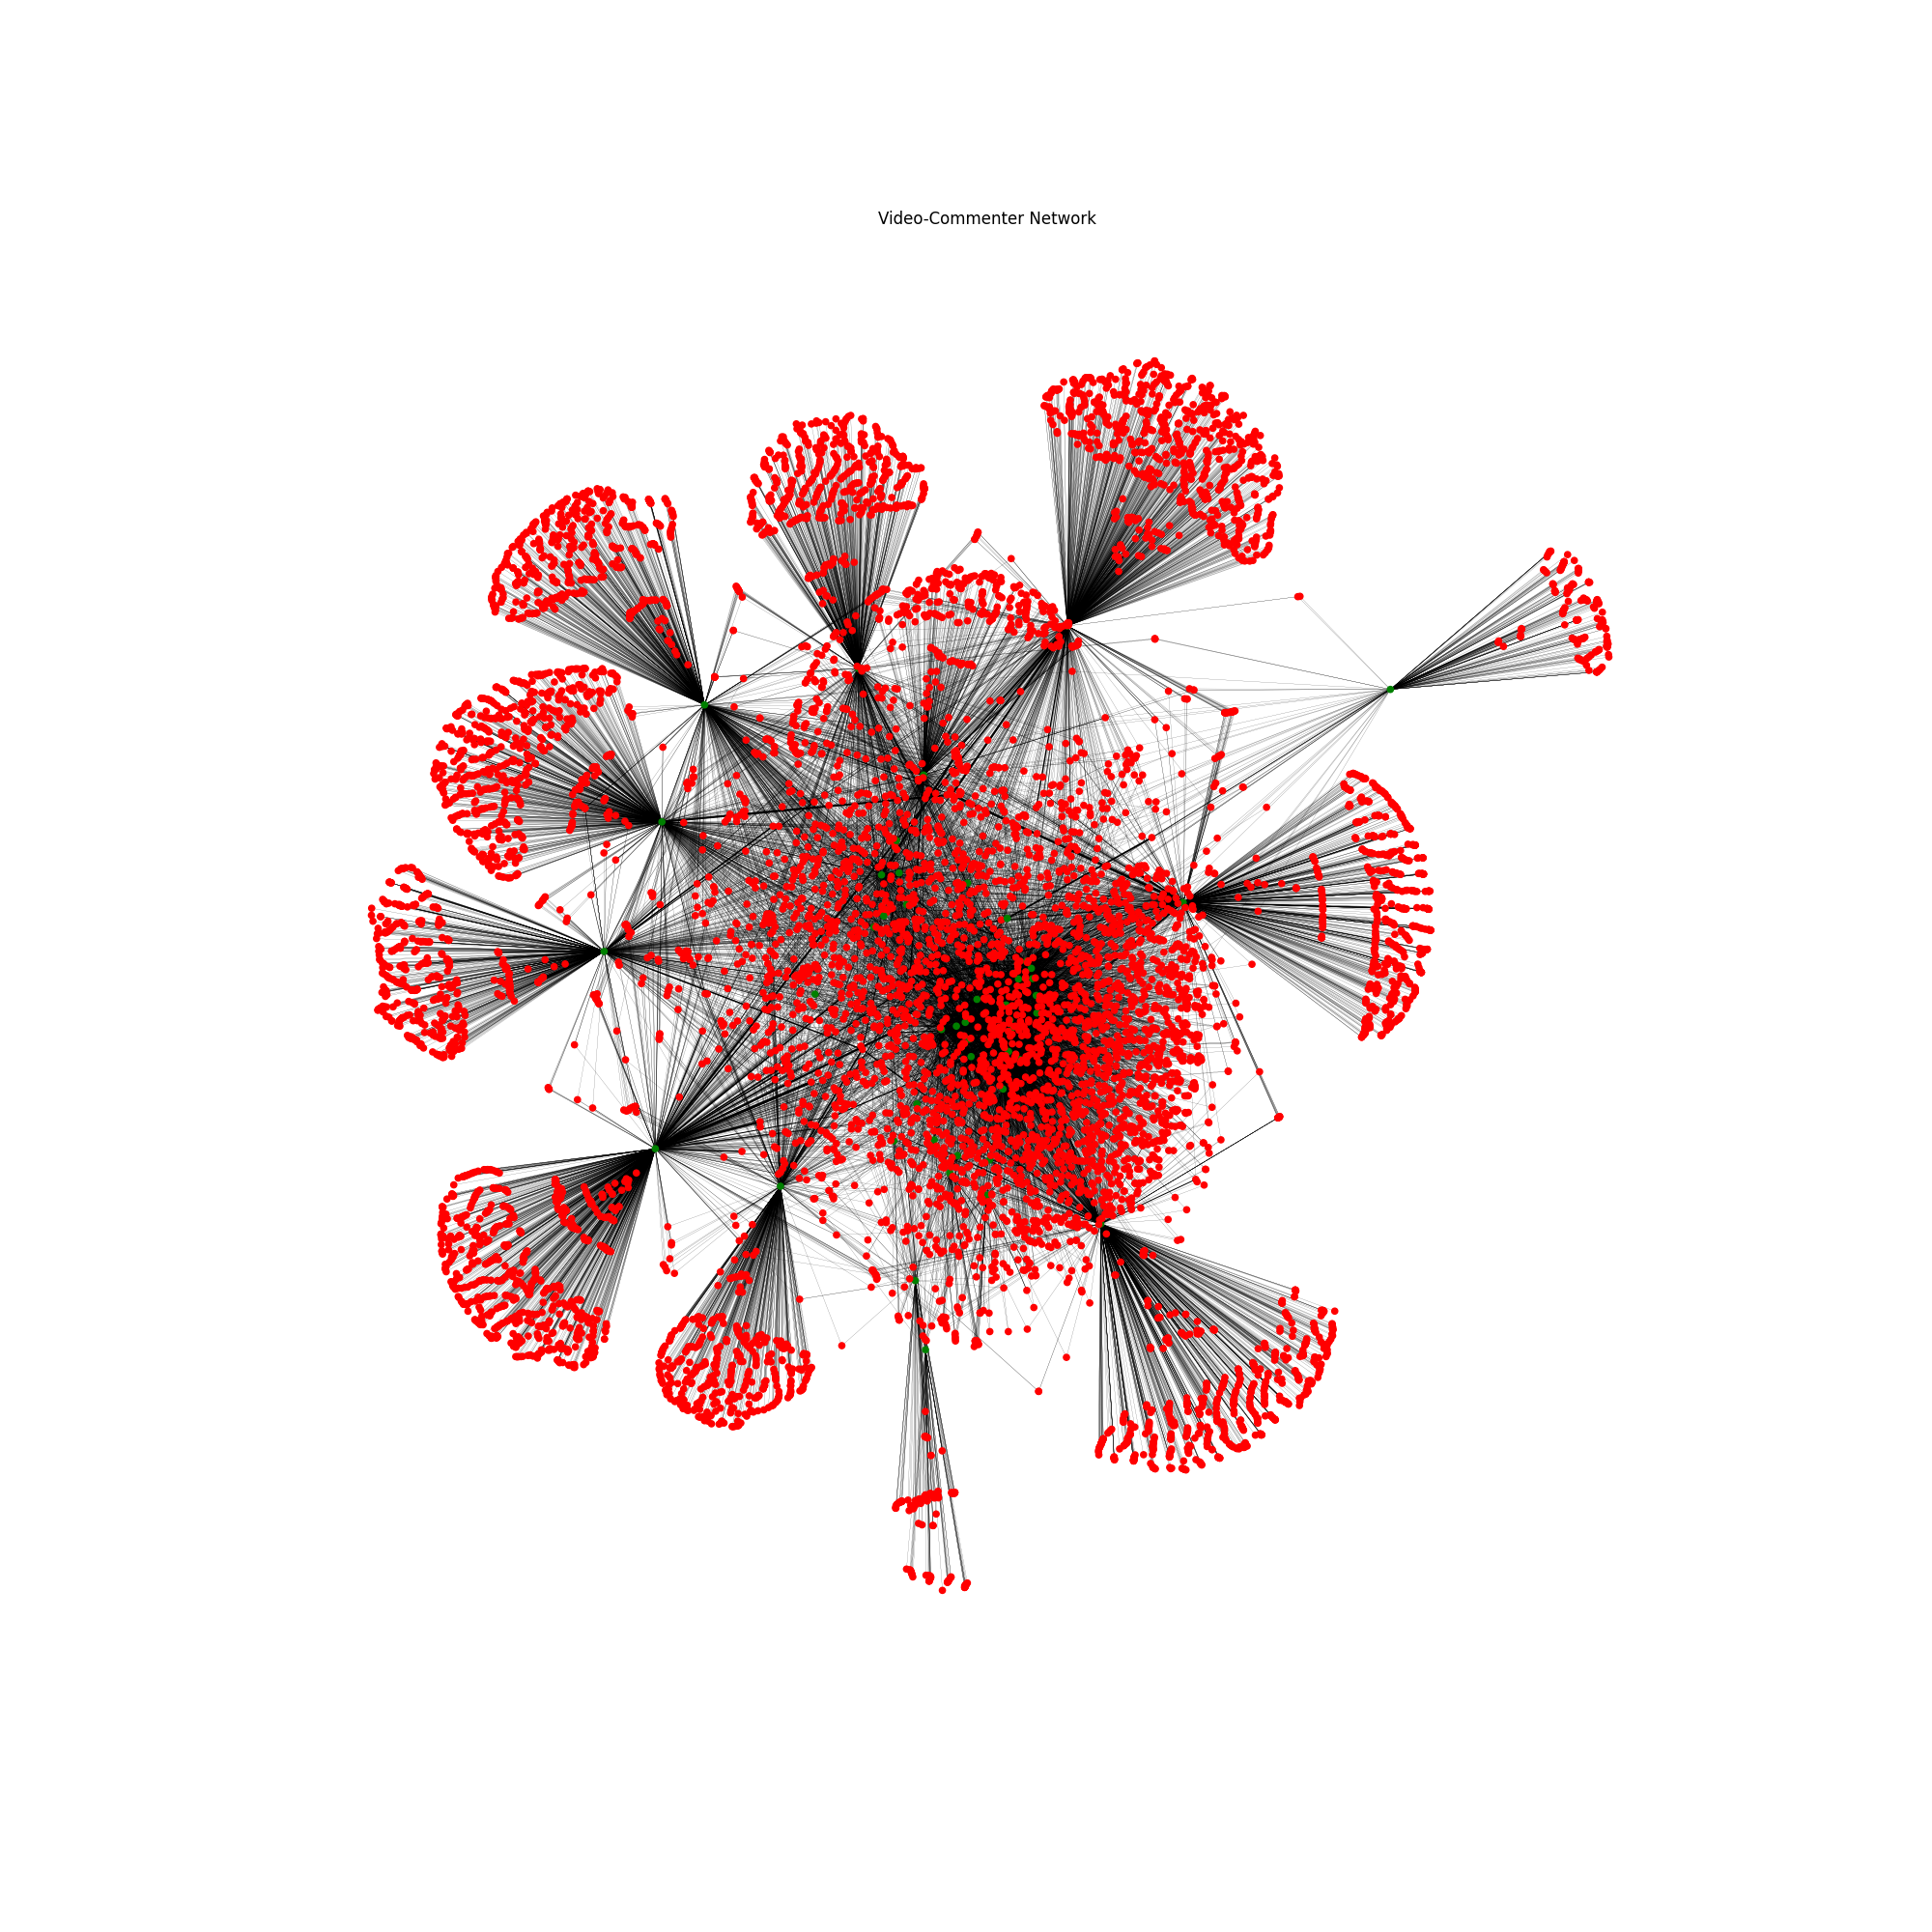
\includegraphics[keepaspectratio,width=0.8\textwidth]{./imgs/felipeneto/felipeneto_video_commenter_network.png}
    \caption[width=\textwidth]{Youtuber 1's Video-Commenter Network}
    \label{fig:ytbr1_vc_net}
\end{figure*}


Then, the BERTopic model was used on the comments made by users situated on the outer clusters, 
followed by the sentiment analysis model, to identify the polarity of the topics.
In Figure~\ref{fig:ytbr1_topics}, the top 10 topics with the most positive and negative topics are 
shown, with the sentiment score greater than 80 percent. 
Of those, it is possible to highlight the first topic of each plot, that has a large number of negative
and positive topics. Also, with the positive topics, it is possible to see that the topics have many
related keywords, such as "amei" and "amo", or "adoro", "gostei".
With the negative topics, the content seems to be more spread, with less related topics. 
The second topic shows the keyword "user", which indicates that many negative comments are made tagging
specific users.

\begin{figure*}[ht]
    \centering
    \begin{minipage}{0.44\textwidth}
        \centering
        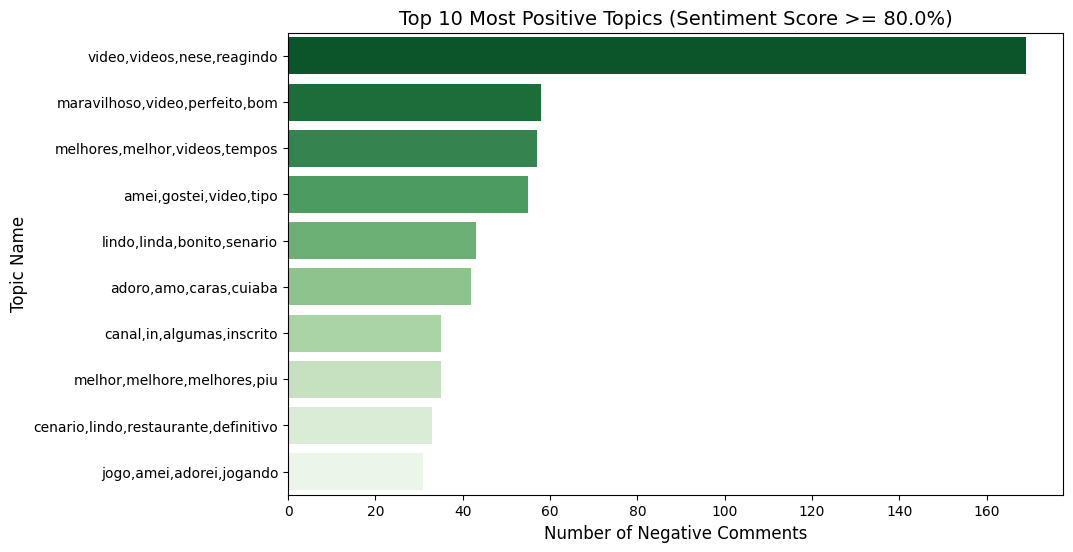
\includegraphics[keepaspectratio,width=\textwidth]{./imgs/felipeneto/most_positive_topics.png}
    \end{minipage}%
    \hspace{0.05\textwidth} % Adjust space between figures if needed
    \begin{minipage}{0.44\textwidth}
        \centering
        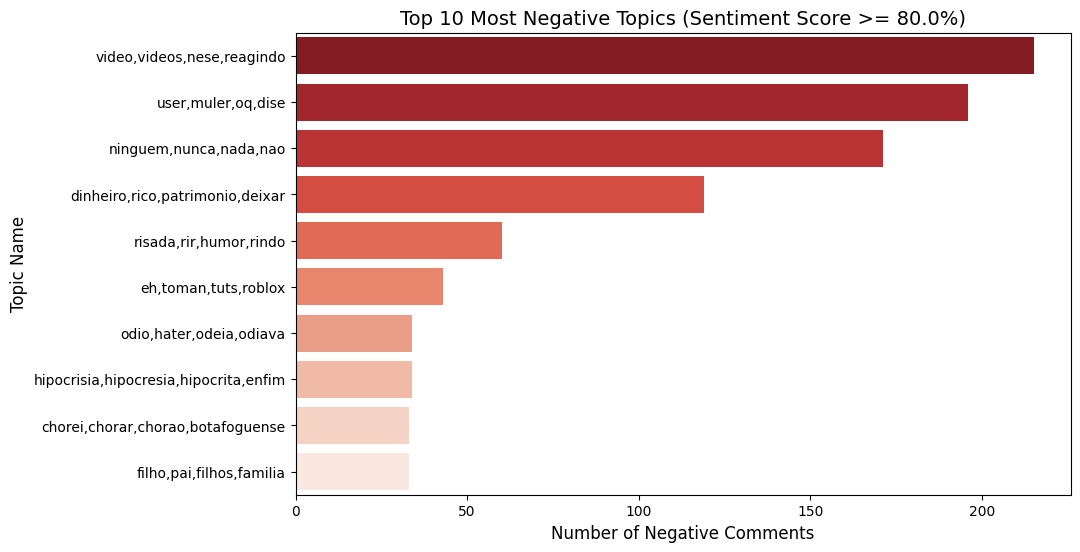
\includegraphics[keepaspectratio,width=\textwidth]{./imgs/felipeneto/most_negative_topics.png}
    \end{minipage}
    \caption{Polarity of the topics}
    \label{fig:ytbr1_topics}
\end{figure*}


\bibliographystyle{sbc}
\bibliography{sbc-template}

\end{document}
